% !TeX root = ../tfg.tex
% !TeX encoding = utf8

\chapter{Símplices y complejos simpliciales}

Los espacios topológicos pueden llegar a ser complicados de estudiar. Los
complejos simpliciales tienen la ventaja de ser estructuras fáciles de estudiar.
Por este motivo, los dotaremos de cierta topología que nos permitirá construir
homeomorfismos a un gran número de espacios topológicos. En este capítulo nos centraremos
en la definición y el estudio de estos objetos en profundidad en la línea de \cite{munkres2018elements}
y lo complementaremos con algunas aportaciones de \cite{lee2010introduction}.

\section{Símplices}
Con la finalidad de generalizar estructuras como el triángulo y el tetraedro, a
finales del siglo XIX nace un nuevo concepto: el símplice. Su sencillez y
propiedades lo convirtieron en una herramienta muy versátil en el estudio de la
topología algebraica, dando lugar a lo que hoy conocemos como homología simplicial.
En esta sección definiremos lo que es un símplice y algunos conceptos asociados
a él que nos serán de gran utilidad en el estudio de dicho campo. Comenzamos recordando
algunos conceptos de la geometría afín.

Como tan sólo será necesario trabajar en el espacio afín usual $N$-dimensional,
lo notaremos simplemente por $\mathbb{R}^{N}$.

\begin{definicion}
	Sea $\{a_{0}, \ldots, a_{p}\}$ un conjunto de puntos en $\mathbb{R}^{N}$.
	Diremos que dicho conjunto es \textbf{afínmente independiente} si para cualesquiera
	$t_{i}\in \mathbb{R}$, las ecuaciones
	\[
	\sum_{i=0}^{p}t_{i}=0 \quad \text{y}\quad \sum_{i=0}^{p}t_{i}a_{i}=0
	\]
	implican que $t_{0}= t_{1}= \ldots = t_{p}$.
\end{definicion}

\begin{definicion}
	Sea $\{a_{0}, \ldots, a_{p}\}$ un conjunto de puntos afínmente independiente.
	Definimos el \textbf{plano afín} $P$ generado por $\{a_{0}, \ldots, a_{p}\}$ como
	el conjunto de puntos $x \in \mathbb{R}^{N}$ tales que
	\[
	x = \sum_{i=0}^{p}t_{i}a_{i}= a_{0}+ \sum_{i=1}^{p}t_{i}(a_{i}- a_{0})
	\]
	para algunos $t_{1}, \ldots, t_{p}\in \mathbb{R}$. Diremos entonces que $P$ es
	el plano que pasa por $a_{0}$ paralelo a los vectores $a_{i}- a_{0}$, $i \in \{
	1, \ldots, p\}$.
\end{definicion}

Nótese que la transformación afín $T$ de $\mathbb{R}^{N}$ tal que
$T(x) = x - a_{0}$ es una traslación que lleva el plano $P$ al subespacio
vectorial de $\mathbb{R}^{N}$ con base
$a_{1}-a_{0}, a_{2}-a_{0}, \ldots, a_{p}-a_{0}$. Si componemos dicha transformación
con una aplicación lineal que lleve cada vector $a_{1}-a_{0}, a_{2}-a_{0}, \ldots
, a_{p}-a_{0}$ a los primeros $N$ vectores de la base usual, obtenemos una
transformación afín $S: P \rightarrow \R^{N}\times \{0\}$ tal que
$S(a_{i}) = (0, \overset{i-1}{\ldots}, 0, 1, 0, \overset{i+1}{\ldots}, 0)$ con
$i \in \{1, \ldots, p\}$.

\begin{definicion}
	\label{def:simplex} Sea $\{a_{0}, \ldots, a_{p}\}$ un conjunto de puntos afínmente
	independiente en $\mathbb{R}^{N}$. Definimos el \textbf{p-símplice} o \textbf{símplice}
	$\sigma = [a_{0}, \ldots, a_{p}]$ generado por $a_{0}, \ldots, a_{p}$ como el
	conjunto de todos los $x \in \mathbb{R}^{N}$ tales que
	\[
	x=\sum_{i=0}^{p}t_{i}a_{i}\quad \text{y}\quad \sum_{i=0}^{p}t_{i}=1
	\]
	con $t_{i}\geq 0$, $i \in \{0, 1, \ldots, p\}$. Diremos que $t_{i}$ es la
	\textbf{$i$-ésima coordenada baricéntrica} de $x$ respecto a $a_{0}, a_{1}, \ldots
	, a_{p}$.
\end{definicion}

\begin{proposicion}
	Sea $\sigma$ un $k$-símplice definido como en \ref{def:simplex}. Entonces, para
	cualquier $p \in \sigma$, las coordenadas baricéntricas $t_{0}, \ldots, t_{k}$
	de $p$ están determinadas de manera única.
\end{proposicion}
\begin{proof}
	Por definición, cualquier punto arbitrario $p \in \sigma$ puede escribirse
	como una combinación convexa de los puntos $a_{i}$. Esto garantiza la existencia
	de una solución (no negativa) al sistema lineal
	\[
	At= \left(
	\begin{array}{ccc}
		a_{01} & \cdots & a_{k1} \\
		\vdots & \ddots & \vdots \\
		a_{0N} & \cdots & a_{kN} \\
		1      & \cdots & 1
	\end{array}
	\right) \left(
	\begin{array}{c}
		t_0    \\
		\vdots \\
		t_k
	\end{array}
	\right) = \left(
	\begin{array}{c}
		p_1    \\
		\vdots \\
		p_N    \\
		1
	\end{array}
	\right) = p^{*},
	\]
	donde $A$ es la matriz que contiene a los $a_{i}$ como columnas, extendidos
	con un $1$ en la última fila para incorporar la condición de que la suma de
	$t_{i}$ sea igual a $1$, asegurando que estamos considerando combinaciones convexas.
	
	Para demostrar la unicidad, supongamos la existencia de otro vector $t'$ tal
	que $A t'= p^{*}$. Esto lleva a $A(t - t' ) = 0$. Supongamos que
	$A(t - t') = A v = 0$, donde $v = t - t'$. Esto implica que para
	$v_{i}= t_{i}- t_{i}'$ para todo $i \in \{0, \ldots, k\}$
	\[
	\sum_{i=0}^{k}v_{i}\cdot \left(
	\begin{array}{c}
		a_{0i} \\
		\vdots \\
		a_{ki} \\
		1
	\end{array}
	\right) = 0,
	\]
	lo que lleva a que $v_{0}= v_{1}= \cdots = v_{k}= 0$, debido a la independencia
	lineal de las columnas de $A$. En consecuencia, $t= t'$, demostrando así que
	las coordenadas baricéntricas son únicas para cualquier punto $p$ en $\sigma$.
\end{proof}

Los puntos $a_{0}, \ldots, a_{p}$ que generan $\sigma$ los llamaremos \textbf{vértices}
de $\sigma$ y al número $p$ lo llamaremos la \textbf{dimensión} de $\sigma$, que
notaremos por $\dim \sigma$.

\begin{definicion}
	Sea $\sigma=[a_{0}, \ldots, a_{p}]$ un símplice. Una \textbf{cara de dimensión
		$p$} de $\sigma$ será cualquier símplice generado por un subconjunto no vacío de
	$\{a_{0}, \ldots, a_{p}\}$.
\end{definicion}
En particular, la cara de $\sigma$ generada por
$a_{0}, \ldots, a_{i-1}, a_{i+1}, \ldots, a_{p}$ la llamamos la \textbf{cara
	opuesta} de $a_{i}$, $i \in \{0, \ldots, p\}$. Las caras de $\sigma$ diferentes de
$\sigma$ diremos que son \textbf{caras propias} de $\sigma$ y la unión de todas
ellas la llamaremos el \textbf{borde} de $\sigma$ y lo notaremos $\text{Bd}\ \sigma$.
Finalmente, definimos el \textbf{interior} de $\sigma$, $\interior \sigma$, como
el conjunto de puntos de $\sigma$ que no pertenecen a su borde.

En ocasiones, para dos símplices $\sigma$ y $\tau$, escribiremos
$\tau \preceq \sigma$ si $\tau$ es cara de $\sigma$. En caso de ser cara propia,
lo notaremos por $\tau \prec \sigma$.

\begin{figure}[h]
	\begin{subfigure}
		{.24\textwidth}
		\centering
		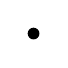
\begin{tikzpicture}
			% 3-símplice
			\node[fill, circle, inner sep=1.5pt] (n0) at (0.0, 0.0) {}; % root
			
			% DRAW NODES
			\draw (n0);
		\end{tikzpicture}
		\caption{0-símplice}
	\end{subfigure}
	\hfill
	\begin{subfigure}
		{.24\textwidth}
		\centering
		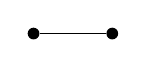
\begin{tikzpicture}
			% 3-símplice
			\node[fill, circle, inner sep=1.5pt] (n0) at (0.0, 0.0) {}; % root
			\node[fill, circle, inner sep=1.5pt] (n1) at (1.0, 0.0) {}; % extreme
			
			% DRAW TREE
			\path[draw] (n0)--(n1);
			
			% DRAW NODES
			\draw (n0); \draw (n1);
		\end{tikzpicture}
		\caption{1-símplice}
	\end{subfigure}
	\hfill
	\begin{subfigure}
		{.24\textwidth}
		\centering
		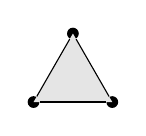
\begin{tikzpicture}
			% 3-símplice
			\node[fill, circle, inner sep=1.5pt] (n0) at (0.0, 0.0) {}; % root
			\node[fill, circle, inner sep=1.5pt] (n1) at (1.0, 0.0) {}; % extreme
			\node[fill, circle, inner sep=1.5pt] (n2) at (0.5, 0.87) {}; % extreme
			
			% DRAW TREE
			\fill[fill=gray!20] (n0.center)--(n1.center)--(n2.center); \path[draw] (n0)--(n1);
			\path[draw] (n1)--(n2); \path[draw] (n2)--(n0);
			
			% DRAW NODES
			\draw (n0); \draw (n1); \draw (n2);
		\end{tikzpicture}
		\subcaption{2-símplice}
	\end{subfigure}
	\hfill
	\begin{subfigure}
		{.24\textwidth}
		\centering
		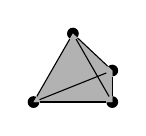
\begin{tikzpicture}
			% 3-símplice
			\node[fill, circle, inner sep=1.5pt] (n0) at (0.0, 0.0) {}; % root
			\node[fill, circle, inner sep=1.5pt] (n1) at (1.0, 0.0) {}; % extreme
			\node[fill, circle, inner sep=1.5pt] (n2) at (0.5, 0.87) {}; % extreme
			\node[fill, circle, inner sep=1.5pt] (n3) at (1.0, 0.4) {}; % inside
			
			% DRAW TREE
			\fill[fill=gray!60] (n0.center)--(n1.center)--(n2.center); \fill[fill=gray!60]
			(n0.center)--(n2.center)--(n3.center); \fill[fill=gray!60] (n0.center)--(n1.center)--(n3.center);
			\fill[fill=gray!60] (n3.center)--(n1.center)--(n2.center); \path[draw] (n0)--(n1);
			\path[draw] (n1)--(n2); \path[draw] (n2)--(n0); \path[draw] (n0)--(n3);
			\path[draw] (n1)--(n3); \path[draw] (n2)--(n3);
			
			% DRAW NODES
			\draw (n0); \draw (n1); \draw (n2); \draw (n3);
		\end{tikzpicture}
		\caption{3-símplice}
	\end{subfigure}
	\caption{Símplices de dimensión $0$, $1$, $2$ y $3$}
	\label{fig:simplex}
\end{figure}
\begin{proposicion}
	\label{prop:union-disjunta-simplices} Si $\sigma$ es un símplice, entonces es
	unión disjunta del interior de todas sus caras.
\end{proposicion}
\begin{proof}
	Sea $x$ un elemento del símplice $\sigma = [a_{0},\ldots,a_{p}]$ y sean $t_{0},
	\ldots ,t_{p}$ sus coordenadas baricéntricas. Consideremos ahora $\sigma_{k}$
	el símplice resultante de eliminar los vértices cuya coordenada tenía valor
	nulo. Esto es, tomamos el símplice $\sigma_{k}= [a_{i_1}, \ldots, a_{i_k}]$
	donde $t_{i_s}> 0$ para todo $s \in \{1, \ldots, k\}$. Por la construcción de $\sigma
	_{k}$, tenemos que $x$ pertenece a su interior.
	
	Ahora sabemos que todo punto de un símplice pertenece al interior de una cara.
	Finalmente, la unicidad de las coordenadas baricéntricas nos garantiza que la
	unión del interior de dos caras es disjunta.
\end{proof}

Dado un símplice $\sigma$ podemos definir un orden sobre sus vértices. Dos
órdenes de $\sigma$ los consideraremos equivalentes si podemos pasar de uno a
otro con un número par de permutaciones. Así, los ordenamientos posibles para
los vértices de $\sigma$ se pueden agrupar en dos clases de equivalencia
distintas, que definimos como las \textbf{orientaciones del símplice} $\sigma$.

\begin{definicion}
	Decimos que un símplice $\sigma = [a_{0}, a_{1}, \ldots, a_{p}]$ está \textbf{orientado}
	si se le ha asignado una de estas orientaciones. Utilizaremos $[a_{0}a_{1}\ldots
	a_{p}]$ para denotar la clase de equivalencia dada por la orientación $a_{0}< a
	_{1}< \cdots < a_{p}$ del símplice generado por los vértices $a_{0},a_{1},\ldots
	, a_{p}$.
\end{definicion}

\section{Complejos simpliciales}

La importancia de los complejos simpliciales reside en su capacidad para
descomponer espacios topológicos en componentes manejables, permitiendo un análisis
detallado de su estructura. Al considerar la forma en que estos símplices se
conectan y orientan entre sí, los complejos simpliciales facilitarán la definición
de cadenas y ciclos simpliciales que serán indispensables en el estudio de la homología
simplicial.

\begin{definicion}
	Un \textbf{complejo simplicial} (finito) $K$ en $\mathbb{R}^{N}$ es una
	colección (finita) de símplices en $\mathbb{R}^{N}$ tal que:
	\begin{enumerate}
		\item Toda cara de un símplice de $K$ está en $K$.
		
		\item La intersección de cualesquiera dos símplices de $K$ o es el vacío o es
		una cara de ambos símplices.
	\end{enumerate}
\end{definicion}
\begin{nota}
	Si bien los complejos simpliciales se pueden formular sin la restricción de finitud,
	nosotros trabajaremos principalmente en el caso finito por simplicidad en
	algunos resultados.
\end{nota}

\begin{figure}
	\centering
	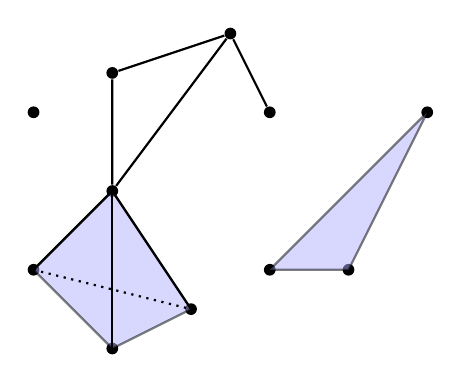
\begin{tikzpicture}
		% Vértices
		\node[fill, circle, inner sep=1.5pt] (A) at (0,1) {}; \node[fill, circle,
		inner sep=1.5pt] (B) at (1,0) {}; \node[fill, circle, inner sep=1.5pt] (C) at
		(2,0.5) {}; \node[fill, circle, inner sep=1.5pt] (D) at (1,2) {};
		
		\node[fill, circle, inner sep=1.5pt] (E) at (1,3.5) {}; \node[fill, circle, inner
		sep=1.5pt] (F) at (2.5,4) {}; \node[fill, circle, inner sep=1.5pt] (G) at (3,3)
		{};
		
		\node[fill, circle, inner sep=1.5pt] (H) at (0,3) {};
		
		\node[fill, circle, inner sep=1.5pt] (I) at (3,1) {}; \node[fill, circle, inner
		sep=1.5pt] (J) at (5,3) {}; \node[fill, circle, inner sep=1.5pt] (K) at (4,1)
		{};
		
		% Dibujar el 3-simplex
		\draw[thick, fill=blue!30, opacity=0.5] (A.center) -- (B.center) -- (C.center)
		-- (D.center) -- cycle; \draw[thick] (A.center) -- (D.center); \draw[thick]
		(B.center) -- (D.center); \draw[thick] (C.center) -- (D.center);
		
		% Línea punteada
		\draw[dotted, thick] (A.center) -- (C.center);
		
		% Dibujar el 1-simplex
		\draw[thick] (D) -- (E) -- (F) -- (G); \draw[thick] (D) -- (F);
		
		% Dibujar el 2-simplex
		\draw[thick, fill=blue!30, opacity=0.5] (I.center) -- (J.center) -- (K.center)
		-- cycle;
		
		% Dibujar 0-simplex
		\fill[black] (H) circle (2pt);
	\end{tikzpicture}
	\caption{Visualización de un complejo simplicial.}
\end{figure}

En ciertas ocasiones puede ser interesante saber si dada una colección cualquiera
de símplices, esta es un complejo simplicial o no. Para ello, el siguiente lema
nos puede ser de utilidad.

\begin{lema}
	Una colección $K$ de símplices es un complejo simplicial si, y sólo si, se cumplen
	las siguientes condiciones:
	\begin{enumerate}
		\item Toda cara de un símplice de $K$ está en $K$.
		
		\item La intersección dos a dos del interior de los símplices de $K$ es vacía.
	\end{enumerate}
\end{lema}
\begin{proof}
	Primero, asumamos que $K$ es un complejo simplicial. Dados dos símplices $\sigma
	, \tau \in K$ veamos que si el interior de ambos tiene un punto $x$ en común,
	entonces $\sigma = \tau$. Sea $s = \sigma \cap \tau$ y considero $x \in s$. Si
	$s$ fuera una cara propia de $\sigma$, entonces $x$ pertenecería a la frontera
	de $\sigma$, lo cual no se cumple ya que $x$ pertenece al interior de $\sigma$.
	Por tanto $s = \sigma$. De manera análoga, $s = \tau$, luego $\sigma = \tau$.
	
	Asumamos ahora que se cumplen \textit{(1)} y \textit{(2)}. Queremos ver que si
	el conjunto $\sigma \cap \tau \neq \emptyset$, dicha intersección es la cara
	$\sigma'$ de $\sigma$ generada por los vértices $b_{0},\ldots,b_{m}$ de
	$\sigma$ que están en $\tau$. Primero, $\sigma' \subset \sigma \cap \tau$ por
	ser $\sigma \cap \tau$ convexa y contener a $b_{0}, \ldots, b_{m}$. Para la otra
	inclusión supongamos que $x \in \sigma \cap \tau$. Esto implica que
	$x \in \interior s \cap \interior t$ para alguna cara $s$ de $\sigma$ y alguna
	cara $t$ de $\tau$. Se sigue de \textit{(2)} que $s = t$ por lo que los
	vértices de $s$ están en $\tau$ y por definición, son elementos del conjunto $\{
	b_{0}, \ldots, b_{m}\}$. Concluimos entonces que $s$ es una cara de $\sigma'$,
	lo que implica que $x \in \sigma'$, como queríamos ver.
\end{proof}

\begin{definicion}
	Si $L$ es una subcolección del complejo simplicial $K$ que contiene todas las caras
	de sus elementos, entonces $L$ es un complejo simplicial que llamaremos
	\textbf{subcomplejo} de $K$.
\end{definicion}
\begin{definicion}
	Sea $K$ un complejo simplicial. Diremos \textbf{p-esqueleto} de $K$ al subcomplejo
	formado por todas las caras de $K$ cuya dimensión sea menor o igual que $p$.
	Lo denotaremos por $K^{(p)}$. En particular, $K^{(0)}$ lo llamaremos el
	\textbf{conjunto de vértices} de $K$.
\end{definicion}
\begin{definicion}
	Sea $K$ un complejo simplicial de $\mathbb{R}^{N}$ y sea $|K|$ el subconjunto de
	$\mathbb{R}^{N}$ tal que $|K|$ es la unión de todos los símplices de $K$.
	Definimos el \textbf{politopo} o \textbf{espacio subyacente} de $K$ como el
	espacio topológico $(|K|, \mathcal{T})$ donde los abiertos de $\mathcal{T}$
	son aquellos $O \subseteq |K|$ tal que $O \cap \sigma$ es abierto en $\sigma$
	con la topología inducida de $\mathbb{R}^{N}$ para todo $\sigma \in K$.
\end{definicion}

Veamos que en efecto $(|K|, \mathcal{T})$ es un espacio topológico. $\emptyset, |
K| \in \mathcal{T}$ ya que son abiertos trivialmente en $\sigma$, pues
$\emptyset \cap \sigma = \emptyset$ y $|K| \cap \sigma = \sigma$ para todo
$\sigma \in K$. Si $O_{1}, O_{2}\in \mathcal{T}$, entonces $O_{1}\cap \sigma$, $O
_{2}\cap \sigma$ son abiertos en $\sigma$ luego $(O_{1}\cap O_{2}) \cap \sigma =
(O_{1}\cap \sigma) \cap (O_{2}\cap \sigma)$ es abierto en $\sigma$ para todo $\sigma
\in K$. Por tanto $O_{1}\cap O_{2}\in \mathcal{T}$. Finalmente, consideremos una
familia $\{O_{i}\}_{i \in I}\subset \mathcal{T}$ donde $I$ es un conjunto de
índices. Para cada $\sigma \in K$,
$(\cup_{i \in I}O_{i}) \cap \sigma = \cup_{i \in I}(O_{i}\cap \sigma)$ que
efectivamente es una unión arbitraria de abiertos de $\sigma$. En consecuencia,
$\cup_{i \in I}O_{i}\in \mathcal{T}$.

En general, la topología de $|K|$ es más fina que la inducida de la topología usual
de $\R^{N}$. Si $A$ es cerrado en $|K|$ con la topología inducida de la usual, $A
=B \cap |K|$ para algún cerrado $B$ de $\R^{N}$ y por tanto $B \cap \sigma$ sería
cerrado en $\sigma$ para cada símplice $\sigma$ de $K$. Como consecuencia, $B \cap
|K|=A$ es cerrado en $|K|$ con la topología $\mathcal{T}$ definida anteriormente.
No obstante, la otra inclusión no tiene por qué cumplirse:

\begin{ejemplo}
	Consideremos el complejo no finito $K$ en $\R$ cuyos símplices son todos los intervalos
	$[m,m+1]$ con $m \in \Z \backslash \{0\}$, todos los intervalos de la forma
	$[1/( n+1), 1/n]$ donde $n \in \N$ y todas sus respectivas caras. Como resultado
	tenemos que $|K| = \R$, donde $F = \{1/n : n \in \N\}$ es cerrado en nuestra
	topología $\mathcal{T}$ pero no en la inducida por la usual. Dicho de otra forma,
	$\R \backslash F$ es abierto en $\mathcal{T}$ pero no en la usual.
\end{ejemplo}

Si no hay lugar a confusión, simplemente notaremos al politopo de $K$ por $|K|$ y
lo llamaremos el \textbf{poliedro} $|K|$.

A continuación, mencionemos algunas propiedades relevantes de este espacio topológico.
Para ello fijemos un complejo simplicial finito $K$ en $\R^{N}$.

\begin{proposicion}
	Sea $K$ un complejo simplicial finito. Entonces el poliedro $|K|$ es compacto.
\end{proposicion}
\begin{proof}
	Si $K$ es un complejo simplicial, sus símplices son conjuntos cerrados y
	acotados. En consecuencia, $|K|$ es unión finita de conjuntos cerrados y
	acotados, luego es cerrado y acotado en $\R^{N}$. Por lo tanto, es compacto.
\end{proof}
%\begin{proposicion}
%	Si el poliedro \(|K|\) es conexo, entonces es arco conexo.
%\end{proposicion}
%\begin{proof}
%	DEMOSTRAR DE 2.1A DL TFG ANTIGUO...
%\end{proof}
\begin{proposicion}
	Sea $K$ un complejo simplicial. \label{prop:simpl-soporte} Si $x \in |K|$, entonces
	existe un único símplice en $K$ tal que $x$ pertenece a su interior.
\end{proposicion}
\begin{proof}
	Si $x \in |K|$, entonces existe algún símplice $\sigma$ de $K$ tal que
	$x \in \sigma$. Por la \autoref{prop:union-disjunta-simplices}, $x$ pertenece
	al interior de alguna cara $\tau$ de $\sigma$. Supongamos ahora que existe otro
	símplice $\rho$ de $K$ tal que $x \in \interior \rho$. Por consiguiente, si $x
	\in \interior \rho \cap \interior \tau$, entonces $x$ pertenecería a una cara
	común $\mu$ de $\rho$ y $\tau$. Esto es, $\mu = \rho \cap \tau$. Ahora si $\rho
	\neq \mu$, el elemento $x$ debería tener alguna coordenada baricéntrica nula
	respecto a los vértices de $\rho$, en contradicción con que $x$ pertenece al interior
	de $\rho$. En consecuencia, $\rho = \mu$. De manera análoga obtenemos
	$\tau = \mu$ y por tanto, $\rho = \tau$.
\end{proof}
\begin{definicion}
	Sea $K$ un complejo simplicial y sea $x \in |K|$. Llamaremos \textbf{símplice
		soporte de $x$} al único símplice que contiene a $x$ en su interior y lo notaremos
	por $\sop(x)$.
\end{definicion}
\begin{corolario}
	\label{cor:simpl-soporte} Sean $\sigma, \tau$ símplices de $K$ tal que $\interior
	\sigma \cap \tau$ es no vacía. Entonces $\sigma$ es una cara de $\tau$.
\end{corolario}
\begin{proof}
	Consideremos $x \in \interior \sigma \cap \tau$. Por la
	\autoref{prop:union-disjunta-simplices} sabemos que $\tau$ es la unión de
	todas sus caras lo que implica que existe una cara $\mu$ de $\tau$ cuyo
	interior contiene a $x$. Por lo tanto,
	$x \in \interior \mu \cap \interior \sigma$ y como consecuencia de la
	\autoref{prop:simpl-soporte}, $\mu = \sigma$.
\end{proof}
\begin{lema}
	\label{lem:cont_poly} Sea $K$ un complejo simplicial y $X$ un espacio topológico.
	Una aplicación $f: |K| \rightarrow X$ es continua si, y sólo si, $f|_{\sigma}$
	es continua para cada $\sigma \in K$.
\end{lema}
\begin{proof}
	Si $f$ es continua, también lo es $f|_{\sigma}$ por ser $\sigma$ un subespacio
	de $K$. Supongamos ahora que $f|_{\sigma}$ es continua para cada $\sigma \in K$.
	Si $C$ es un cerrado de $X$, $f^{-1}(C) \cap \sigma = f|_{\sigma}^{-1}(C)$ es un
	cerrado en $\sigma$ por la continuidad de $f|_{\sigma}$. Concluimos que
	$f^{-1}(C)$ es cerrado en $|K|$ por definición.
\end{proof}
\begin{definicion}
	Un espacio topológico $X$ es \textbf{triangulable} si existe un complejo
	simplicial $K$ cuyo espacio subyacente es homeomorfo a $X$. Diremos entonces que
	el homeomorfismo $h: |K| \rightarrow X$ es una \textbf{triangulación}.
\end{definicion}

\section{Celdas y CW-complejos}

A continuación presentamos una generalización del concepto de complejo
simplicial, propuesta por J.H.C. Whitehead en \cite{MR0030759}. Los CW-complejos
reemplazan la estructura simplicial tradicional por estructuras homeomorfas a bolas
abiertas, facilitando el estudio de una gama más amplia de espacios topológicos.

Iniciaremos esta sección estableciendo la notación que utilizaremos. Denotaremos
la \textbf{bola abierta} centrada en $x_{0}$ y de radio $r$ en el espacio
$\mathbb{R}^{N}$ con la topología usual por el conjunto
$B_{r}(x_{0}) = \{ x \in \R^{N} : \| x - x_{0} \| < r \}$. Además, para
cualquier subconjunto $U$ de $\R^{N}$, definiremos su \textbf{clausura} como
$\overline{U}$ y su \textbf{frontera} como $\bd U$. Por último, la \textbf{esfera
	unidad} de dimensión $n$ será representada simplemente como $\sphere^{n-1}$.

\begin{definicion}
	Sea $X$ un espacio topológico. Diremos que $X$ es una \textbf{celda} abierta (cerrada)
	de dimensión $p$ o $p$-celda si $X$ es homeomorfo a la bola unidad abierta (cerrada)
	de dimensión $p$.
\end{definicion}

Sería interesante disponer de resultados que nos digan cuándo un subconjunto dado
puede ser una celda. Para ello, recordemos el siguiente resultado de topología básica:

\begin{lema}
	\label{lem:closed-map} Sean $X,Y$ espacios topológicos y sea $f : X \to Y$ una
	aplicación continua entre ellos. Si $X$ es compacto e $Y$ es Hausdorff, entonces
	$f$ es una aplicación cerrada.
\end{lema}

La siguiente proposición será de gran utilidad para ver que los complejos
simpliciales no son más que un caso particular de los CW-complejos.

\begin{proposicion}
	\label{prop:compact-convex-closed-cell} Si $D \subseteq \mathbb{R}^{n}$ es un subconjunto
	convexo compacto con interior no vacío, entonces $D$ es una $n$-celda cerrada
	y su interior es una $n$-celda abierta. De hecho, dado cualquier punto
	$p \in \interior D$, existe un homeomorfismo $F : \overline{B}_{1}(0) \to D$ que
	envía $0$ a $p$, $B_{1}(0)$ a $\interior D$, y $\sphere^{n-1}$ a $\bd D$.
\end{proposicion}
\begin{proof}
	Sea $p$ un punto interior de $D$. Reemplazando $D$ por su imagen bajo la
	traslación $x \mapsto x - p$, podemos suponer que $p = 0 \in \interior D$.
	Entonces existe algún $\varepsilon > 0$ tal que la bola $B_{\varepsilon}(0)$
	está contenida en $D$. Utilizando la dilatación $x \mapsto x/\varepsilon$,
	podemos asumir $B_{1}(0) \subseteq D$.
	\begin{figure}
		\centering
		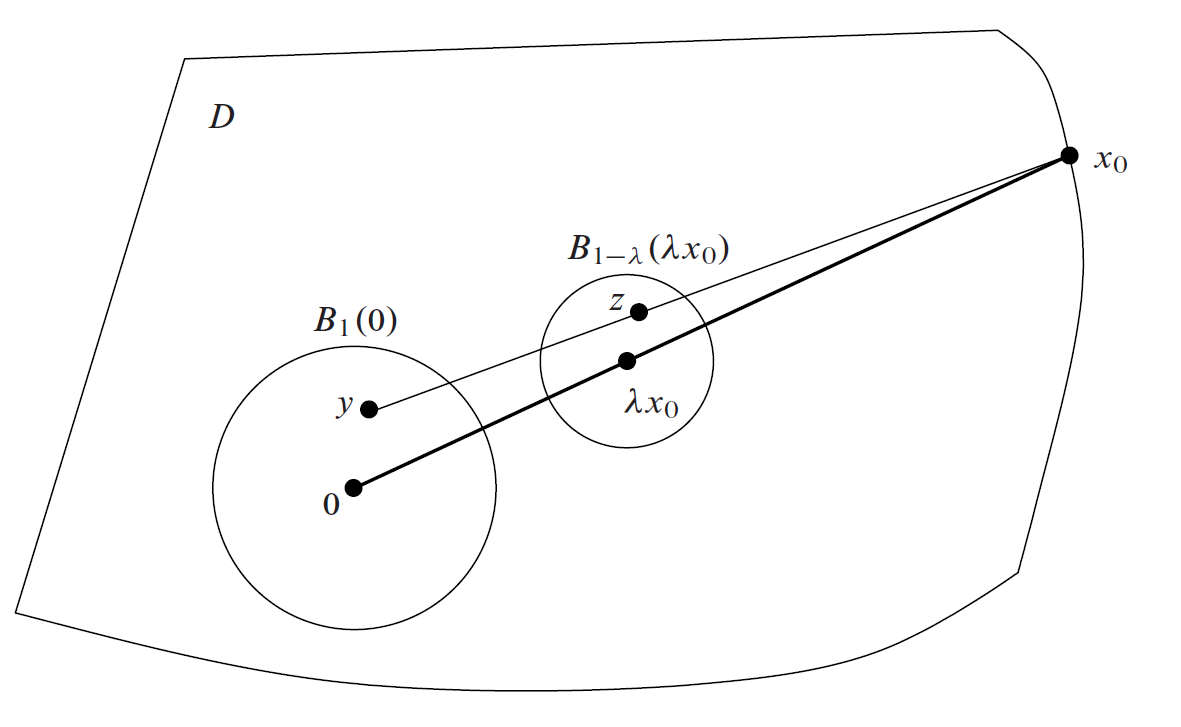
\includegraphics[width=10cm]{img/proof-cell.png}
		\caption{Esquema que muestra la idea de que cada rayo tan sólo tiene un
			punto en la frontera en la demostración de la
			\autoref{prop:compact-convex-closed-cell}. Recurso obtenido de \cite{lee2010introduction}.}
	\end{figure}
	A continuación demostraremos que cada semirrecta cerrada que comienza en el origen
	interseca $\bd D$ en exactamente un punto. Sea $R$ tal semirrecta cerrada. Dado
	que $D$ es compacto, su intersección con $R$ es compacta; por lo tanto, hay un
	punto $x_{0}$ en esta intersección donde la distancia al origen alcanza su
	máximo. Este punto se identifica fácilmente como parte del borde de $D$. Para
	demostrar que solo puede haber un punto así, mostramos que el segmento de línea
	desde $0$ hasta $x_{0}$ consta enteramente de puntos interiores de $D$,
	excepto $x_{0}$ mismo. Cualquier punto en este segmento que no sea $x_{0}$ se puede
	escribir en la forma $\lambda x_{0}$ para $0 \leq \lambda < 1$. Supongamos que
	$z \in B_{1-\lambda}(x_{0})$, y sea $y = (z - \lambda x_{0})/(1 - \lambda)$.
	En consecuencia $|y| < 1$, por lo que $y \in B_{1}(0) \subseteq D$. Como $y$ y
	$x_{0}$ están ambos en $D$ y $z = \lambda x_{0} + (1 - \lambda)y$, se sigue de
	la convexidad que $z \in D$. Así, la bola abierta $B_{1-\lambda}(x_{0})$ está contenida
	en $D$, lo que implica que $\lambda x_{0}$ es un punto interior.
	
	Ahora definamos una aplicación $f : \bd D \to \sphere^{n-1}$ por
	\[
	f(x) = \frac{x}{|x|}.
	\]
	
	En palabras, $f(x)$ es el punto donde el segmento de línea que parte del
	origen hasta $x$ interseca la esfera unidad. Puesto que $f$ es la restricción de
	una aplicación continua, es continua, por lo que la discusión del párrafo anterior
	muestra que es biyectiva. Dado que $\partial D$ es compacto, $f$ es un homeomorfismo
	por el \autoref{lem:closed-map}.
	
	Finalmente, definamos $F : \overline{B}_{1}(0) \to D$ de forma que
	\[
	F(x) =
	\begin{cases}
		|x| f^{-1}\left( \frac{x}{|x|}\right), & x \neq 0; \\
		0,                                     & x = 0.
	\end{cases}
	\]
	Entonces $F$ es continua lejos del origen porque $f^{-1}$ lo es, y también lo es
	en el origen pues la acotación de $f^{-1}$ implica que $F(x) \to 0$ conforme $x
	\to 0$. Geométricamente, $F$ lleva cada segmento de línea radial que conecta $0$
	con un punto $\omega \in \sphere^{n-1}$ linealmente sobre el segmento radial de
	$0$ al punto $f^{-1}(\omega) \in \bd D$. Por convexidad, $F$ toma sus valores en
	$D$. La aplicación $F$ es inyectiva, ya que puntos en rayos distintos van a rayos
	distintos, y cada segmento radial se lleva linealmente a su imagen. Es sobreyectiva
	porque cada punto $y \in D$ está en algún rayo desde $0$. Por el
	\autoref{lem:closed-map}, $F$ es un homeomorfismo.
\end{proof}

\begin{definicion}
	Sea $(X,\mathcal{E})$, donde $X$ es un espacio topológico Hausdorff y
	$\mathcal{E}$ una colección de celdas abiertas. Diremos entonces que que $(X,\mathcal{E}
	)$ es un \textbf{CW-complejo} si se cumple que:
	\begin{enumerate}[font=\bfseries]
		\item[(C)] Para cada $p$-celda $e \in \mathcal{E}$, existe una aplicación
		continua $f_{e} : B^{p} \to X$ de forma que el interior de $B^{p}$ es
		homeomorfo a la celda $e$ y lleva la frontera de $B^{p}$ en una unión
		finita de celdas de dimensión menor a $p$. A dicha función la llamaremos \textbf{función
			característica}.
		
		\item[(W)] Un subconjunto $F$ de $X$ es cerrado si $F \cap \overline{e}$,
		donde $\overline{e}$ denota la clausura de $e$, es cerrado para todo $e \in
		\mathcal{E}$.
	\end{enumerate}
	Normalmente denotaremos al CW-complejo $(X,\mathcal{E})$ simplemente por $X$.
\end{definicion}
\begin{observacion}
	En la formulación original de Whitehead, la primera condición denotaba la
	propiedad de clausura finita. Por otro lado, la segunda condición denotaba que
	la topología empleada era la topología débil (del inglés, \textit{weak}).% Si bien esta formulación nos aleja un poco de la intuición original, es una formulación equivalente.
\end{observacion}

\begin{figure}[h!]
	\centering
	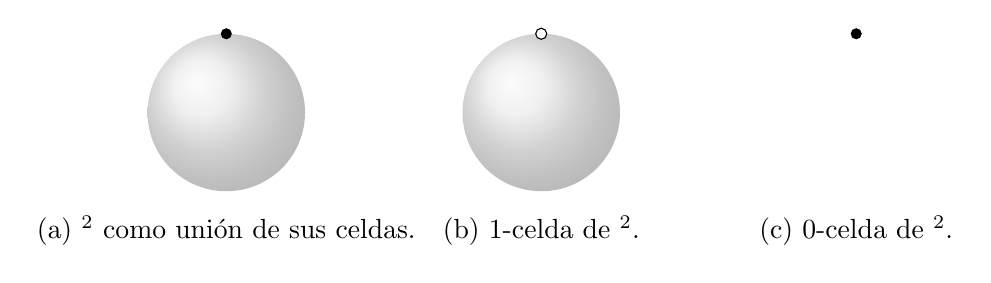
\begin{tikzpicture}
		% Sphere with a dot (0-cell)
		\begin{scope}
			[shift={(0,0)}] \shade[ball color = gray!40, opacity = 0.4] (0,0) circle (1cm);
			\fill (0,1) circle (2pt); \node at (0,-1.5)
			{(a) $\sphere^{2}$ como unión de sus celdas.};
		\end{scope}
		
		% Sphere with a hole
		\begin{scope}
			[shift={(4,0)}] \shade[ball color = gray!40, opacity = 0.4] (0,0) circle (1cm);
			\fill[white] (0,1) circle (2pt); \draw (0,1) circle (2pt); \node at (0,-1.5)
			{(b) $1$-celda de $\sphere^{2}$.};
		\end{scope}
		
		% Dot aligned with the hole
		\begin{scope}
			[shift={(8,0)}] \fill (0,1) circle (2pt); \node at (0,-1.5) {(c) $0$-celda de $\sphere^{2}$.};
		\end{scope}
	\end{tikzpicture}
	\caption{Visualización de un CW-complejo para $\sphere^{2}$.}
\end{figure}

\begin{definicion}
	Sea $X$ un espacio topológico. Diremos que una celda $e \subset X$ es \textbf{regular}
	si admite una función característica que sea un homeomorfismo sobre $\overline{e}$.
	Además, diremos que un CW-complejo es \textbf{regular} si todas sus celdas son
	regulares.
\end{definicion}

Una propiedad importante de los CW-complejos es que mantienen su estructura en
subconjuntos bajo ciertas condiciones razonables.

\begin{definicion}
	Sea $X$ un CW-complejo. Diremos que $Y \subseteq X$ es un \textbf{subcomplejo}
	de $X$ si es unión de celdas de $X$ de forma que si $Y$ contiene una celda,
	entonces también contiene su clausura.
\end{definicion}

\begin{teorema}
	Sea $X$ un CW-complejo y sea $Y$ un subcomplejo de $X$. Entonces $Y$ es
	cerrado en $X$ y, además, es un CW-complejo con la topología y la colección de
	celdas inducidas.
\end{teorema}
\begin{proof}
	Es claro que $Y$ es Hausdorff. Además, por definición tenemos que $Y$ es la unión
	disjunta de sus celdas. Sea $e \subseteq Y$ una celda abierta de $Y$. Como su clausura
	también está contenida en $Y$, entonces existe un número finito de celdas de
	$X$ con intersección no vacía con $\overline{e}$ que, a su vez, son celdas de
	$Y$. En consecuencia, la condición $(C)$ se cumple. Es más, cualquier
	aplicación característica $f_{e} : \to X$ de $X$ lo es también de $Y$ para
	cualquier celda $e \subseteq Y$.
	
	En cuanto a la condición $(W)$, supongamos que $S$ es un subconjunto de $Y$ tal
	que $S \cap \overline{e}$ es cerrado en $\overline{e}$ para toda celda en $Y$.
	Sea ahora $e$ una celda de $X$ que no esté contenida en $Y$. Sabemos que $\overline
	{e}\backslash e$ está contenido en la unión de un número finito de celdas de $X$,
	de las cuales un subconjunto de ellas están contenidas en $Y$. Llamemos a dichas
	celdas $e_{1}, \ldots, e_{n}$. Por consiguiente, $\overline{e}_{1} \cup \cdots
	\cup \overline{e}_{n} \subseteq Y$ y además,
	\[
	S \cap \overline{e}= S \cap (\overline{e}_{1} \cup \cdots \cup \overline{e}_{n}
	) \cap \overline{e}= \left( (S \cap \overline{e}_{1}) \cup \cdots \cap (S \cap
	\overline{e}_{n}) \right) \cap \overline{e},
	\]
	luego $S \cap \overline{e}$ es cerrado en $\overline{e}$. Es decir, $S$ es
	cerrado en $X$ y por tanto en $Y$. Finalmente, concluimos que $Y$ es cerrado
	en $X$ tomando $S = Y$.
\end{proof}

\begin{definicion}
	Sea $X$ un CW-complejo. Diremos que el subespacio $X^{(p)}$ de $X$ es el
	\textbf{$p$-esqueleto} de $X$ si es igual a la unión de todas las celdas de dimensión
	menor o igual que $p$. En particular, es un subcomplejo de dimensión $p$ de $X$.
\end{definicion}

\begin{teorema}
	Sea $X$ un CW-complejo. Entonces las siguientes propiedades son equivalentes:
	\begin{enumerate}
		\item $X$ es conexo por caminos.
		
		\item $X$ es conexo.
		
		\item El $1$-esqueleto de $X$ es conexo.
		
		\item Algún $n$-esqueleto de $X$ es conexo para algún $n$.
	\end{enumerate}
\end{teorema}
\begin{proof}
	Obviamente, $(1) \Rightarrow (2)$ y $(3) \Rightarrow (4)$, por lo que basta con
	demostrar que $(2) \Rightarrow (3)$ y $(4) \Rightarrow (1)$.
	
	Para probar $(2) \Rightarrow (3)$ razonaremos por contrarrecíproco. Supongamos
	que $X^{(1)}= X'^{(1)}\cup X''^{(1)}$ es una unión no conexa del $1$-esqueleto
	de $X$. Veamos por inducción en $n$ que para cada $n > 1$, el $n$-esqueleto
	$X^{(n)}$ puede expresarse como unión no conexa
	$X^{(n)}= X'^{(n)}\cup X''^{(n)}$ tal que $X'^{(n)}\subseteq X'^{(n-1)}$ y
	$X''^{(n)}\subseteq X''^{(n-1)}$ para cada $n$. Supongamos $X^{(n-1)}= X'^{(n-1)}
	\cup X''^{(n-1)}$ es una unión no conexa de $X^{(n-1)}$ para algún $n > 1$.
	Para cada celda $n$-dimensional $e$, la restricción de su aplicación función característica
	$f_{e} \colon D^{n} \to X^{(n)}$ a $\partial D^{n}$ es continua en $X^{(n-1)}$.
	Dado que $\partial D^{n} \cong \sphere^{n-1}$ es conexo, su imagen debe estar contenida
	en uno de los conjuntos $X'^{(n)}$ o $X''^{(n)}$. Por lo tanto, $\overline{f_e(D)}$
	tiene una intersección no trivial con $X'^{(n)}$ o $X''^{(n)}$, pero no con
	ambos. Dividimos las $n$-celdas en dos colecciones disjuntas $\mathcal{E}'$ y $\mathcal{E}
	''$, según si sus clausuras intersecan $X'^{(n-1)}$ o $X''^{(n-1)}$, respectivamente,
	y definimos
	\[
	X'^{(n)}= X'^{(n-1)}\cup \left(\bigcup_{e \in \mathcal{E}'}\overline{f_e(e)}\right
	),\quad X''^{(n)}= X''^{(n-1)}\cup \left(\bigcup_{e \in \mathcal{E}''}\overline
	{f_e(e)}\right).
	\]
	Claramente, $X^{(n)}$ es la unión disjunta de $X'^{(n)}$ y $X''^{(n)}$, y
	ambos conjuntos son no vacíos debido a la hipótesis de inducción.
	
	Ahora, definamos $X' = \bigcup_{n} X'^{(n)}$ y $X'' = \bigcup_{n} X''^{(n)}$.
	Como antes, $X = X' \cup X''$, y ambos conjuntos son no vacíos. Por el mismo argumento
	que arriba, si $e$ es cualquier celda de $X$ de cualquier dimensión, su clausura
	debe estar contenida en uno de estos conjuntos. Así, $X'$ y $X''$ son ambos abiertos
	y cerrados en $X$, lo que implica que $X$ no es conexo.
	
	Para demostrar $(4) \Rightarrow (1)$, supongamos que $X$ es un CW-complejo cuyo
	$n$-esqueleto es conexo para algún $n \geq 0$. Mostremos por inducción en $k$
	que $X^{(k)}$ es conexo por caminos para cada $k \geq n$. Primero, necesitamos
	mostrar que $X^{(n)}$ en sí mismo es conexo por caminos. Si $n = 0$, entonces
	$X^{(n)}$ es discreto y conexo, así que es un conjunto unitario y por lo tanto
	conexo por caminos. En caso contrario, elijamos cualquier punto $x_{0} \in X^{(n)}$
	y consideremos $S_{n}$ la componente de camino de $X^{(n)}$ que contiene a $x_{0}$.
	Para cada celda $e$ de $X^{(n)}$, notemos que $\overline{f_e(e)}$ es la imagen
	continua de un espacio conexo por caminos, así que es conexo por caminos. Por lo
	tanto, si $\overline{f_e(e)}$ tiene una intersección no trivial con la
	componente de camino $S_{n}$, debe estar contenida en $S_{n}$. En consecuencia,
	$S_{n}$ es cerrado y abierto en $X^{(n)}$. Como estamos asumiendo que
	$X^{(n)}$ es conexo, entonces $S_{n} = X^{(n)}$.
	
	Ahora, supongamos que hemos demostrado que $X^{(k-1)}$ es conexo por caminos
	para algún $k > n$ y sea $S_{k}$ la componente de camino de $X^{(k)}$ que
	contiene a $X^{(k-1)}$. Para cada $k$-celda $e$, su clausura
	$\overline{f_e(e)}$ es un subconjunto de $X^{(k)}$ conexo por caminos que
	tiene intersección no trivial con $X^{(k-1)}$ y, por lo tanto, está contenido
	en $S_{k}$. Se sigue que $X^{(k)}= S_{k}$, completando la inducción.
\end{proof}

\begin{lema}
	\label{lem:cw-cl-finite-subcomplex} Sea $X$ un CW-complejo. Entonces la
	clausura de cada celda está contenida en un subcomplejo finito.
\end{lema}
\begin{proof}
	Consideremos cualquier $n$-celda $e \in X$ y probemos el lema por inducción.
	Para el caso $n=0$, $\overline{e}= e$ es trivialmente un subcomplejo finito.
	Supongamos ahora el lema cierto para las celdas de dimensión menor o igual que
	$n$ y veámoslo para $n+1$. Por la condición $(C)$, $\overline{e}\backslash e$
	está contenido en la unión de un número finito de celdas de dimensión menor
	que $n+1$. Dichas celdas están contenidas en subcomplejo finitos por hipótesis
	de inducción. Sin embargo, la unión de dichos subcomplejos finitos con $e$ es de
	hecho un subcomplejo finito que contiene a $\overline{e}$.
\end{proof}

\begin{lema}
	Sea $X$ un CW-complejo. Un subconjunto de $X$ es discreto si, y sólo si, su
	intersección con cada celda es finita.
\end{lema}
\begin{proof}
	Sea $S$ un subconjunto discreto de $X$. Entonces, la intersección de la clausura
	de cada celda $e$ de $X$ con $S$ es un subconjunto discreto de un conjunto compacto,
	luego es finito. En consecuencia, $S \cap e$ también lo es.
	
	Para la otra implicación supongamos que $S$ es un subconjunto cuya
	intersección con cualquier celda es finita. Como la clausura de cada celda está
	contenida en un subcomplejo finito, entonces por hipótesis tenemos que
	$S \cap \overline{e}$ es finito para cada celda $e$ de $X$. Esto significa que
	$S \cap \overline{e}$ es cerrado en $\overline{e}$ y por la condición $(W)$,
	$S$ es cerrado en $X$. Sin embargo, este argumento podemos aplicarlo a
	cualquier subconjunto de $S$, luego todo subconjunto de $S$ es cerrado en $X$.
	Por lo tanto, la topología inducida en $S$ es discreta.
\end{proof}

\begin{teorema}
	Sea $X$ un CW-complejo. Un subconjunto de $X$ es compacto si, y sólo si, es
	cerrado en $X$ y está contenido en un subcomplejo finito.
\end{teorema}
\begin{proof}
	Todo subcomplejo finito de $X$ es compacto pues es unión finita de clausuras de
	celdas, las cuales son compactas. En consecuencia, si $K$ es un subconjunto
	cerrado de $X$ contenido en un subcomplejo finito, entonces es compacto.
	
	Supongamos ahora que $K \subseteq X$ es compacto. Si $K$ intersecara una
	cantidad infinita de celdas, podríamos tomar un punto de cada intersección de forma
	que tuviéramos un subconjunto infinito discreto de $K$, lo cual es imposible. Es
	decir, $K$ está contenido en la unión de un número finito de celdas y por el
	\autoref{lem:cw-cl-finite-subcomplex}, está contenido en un subcomplejo finito.
\end{proof}

\begin{corolario}
	Un CW-complejo es compacto si, y sólo si, es un complejo finito.
\end{corolario}

\begin{proposicion}
	Todo $p$-símplice es una celda cerrada de dimensión $p$.
\end{proposicion}
\begin{proof}
	Inmediato por la \autoref{prop:compact-convex-closed-cell}.
\end{proof}

Una vez discutidas algunas propiedades básicas de los CW-complejos, ya estamos
en condiciones de verificar que efectivamente los complejos simpliciales son CW-complejos.

\begin{proposicion}
	Si $K$ es un complejo simplicial finito, entonces el poliedro $|K|$ junto con
	la colección $\mathcal{E}$ de interiores de los símplices de $K$ forman un CW-complejo.
\end{proposicion}
\begin{proof}
	Supongamos que $K$ es un complejo simplicial finito en $\mathbb{R}^{N}$. La
	condición $(C)$ se obtiene de manera directa a partir de la
	\autoref{prop:compact-convex-closed-cell}.
	
	En cuanto a la propiedad $(W)$, consideremos $F$ como un subconjunto de $|K|$.
	Sea $\{x_{n}\}_{n \in \N}$ una sucesión que converge a $x$ en $|K|$ y sea $U$
	un entorno de $x$. Por la compacidad de $|K|$ y el hecho de que $\mathcal{E}$ es
	un recubrimiento por abiertos de $|K|$, podemos escoger un subrecubrimiento
	finito $e_{1}, \ldots, e_{k}$ tal que
	$x \in U \subseteq \overline{e_1}\cup \ldots \cup \overline{e_k}$.
	
	Fijemos $n_{0} \in \N$ tal que $x_{n_i}\in U$ para todo $n_{i} \geq n_{0}$. Como
	hay un número finito de $e_{j}$ e infinitos $x_{n_i}$, existe una parcial
	convergente $\{x_{n_i}\}_{i \in \mathbb{N}}$ que converge a $x$ contenido en
	algún $\overline{e}_{j}$ para cierto $j \in \{1, \ldots, k\}$. Esto muestra que
	$x \in \overline{e}_{j}$ y, puesto que $x_{n_i}\in F \cap \overline{e_j}$ para
	todo $n_{i} \geq n_{0}$, y $F \cap \overline{e_j}$ es cerrado en $\overline{e_j}$,
	concluimos que $x \in F \cap \overline{e_k}$.
\end{proof}

\section{Aplicaciones simpliciales}

Cuando trabajemos con complejos simpliciales, será interesante tener en cuenta cuándo
las transformaciones entre ellos pueden ser continuas o incluso homeomorfismos.

\begin{lema}
	\label{lem:app-simpl} Sean $K$ y $L$ dos complejos simpliciales y sea $f: K^{(0)}
	\rightarrow L^{(0)}$ una aplicación entre los conjuntos de vértices de $K$ y $L$.
	Supongamos que siempre que los vértices $v_{0}, \ldots, v_{n}$ de $K$ generen
	un símplice en $K$, los puntos $f(v_{0}), \ldots, f(v_{n})$ son vértices de un
	símplice de $L$. Entonces podemos extender $f$ a una aplicación continua
	$|f| :|K| \rightarrow |L|$ tal que
	\[
	x = \sum_{i=0}^{n}t_{i}v_{i}\quad \implies \quad |f|(x) = \sum_{i=0}^{n}t_{i}
	f (v_{i})
	\]
	Llamaremos a $g$ la \textbf{aplicación simplicial} (lineal) inducida por $f$.
\end{lema}
\begin{proof}
	Por hipótesis, los vértices $f(v_{0}), \ldots, f(v_{n})$ generan un símplice
	$\tau$ en $L$. Por ser $K$ un complejo simplicial, la suma de sus coeficientes
	$t_{i}$, con $i \in \{0, \ldots, n\}$, es igual a uno, luego $|f|(x) = \sum_{i=0}
	^{n}t_{i}f(v_{i})$ es un punto de $\tau$. Es decir, $|f|$ es una aplicación lineal
	del símplice $\sigma$ generado por $v_{0}, \ldots, v_{n}$ al símplice $\tau$ generado
	por $f(v_{0}), \ldots, f(v_{n})$. Por ser $|f| : \sigma \rightarrow \tau$
	lineal en un espacio de dimensión finita, entonces es continua.
	
	Ahora tan solo nos queda ver que $|f| :|K| \rightarrow |L|$ es continua. Bien,
	pues por ser $|f| : \sigma \rightarrow \tau$ continua, también lo es
	$|f| : \sigma \rightarrow |L|$. Finalmente por el \autoref{lem:cont_poly},
	$|f| :|K| \rightarrow |L|$ es continua.
\end{proof}

Consideremos las funciones de la forma de $f$ descrita en \ref{lem:app-simpl}. Para
cualquier complejo $K$, existe una aplicación identidad $\id_{K} \colon K \to K$
que corresponde a la aplicación identidad en los vértices. Dadas tres aplicaciones
$f \colon K \to L$, $g \colon L \to M$ y $h : M \to N$, la aplicación compuesta $h
\circ (g \circ f) = (h \circ g) \circ f$, pues es una composición de
aplicaciones de conjuntos que preserva símplices. Por lo tanto, existe una
categoría de complejos simpliciales y estas funciones que denotaremos por
$\Cat{Csim}$.

Por otro lado, veamos que el \autoref{lem:app-simpl} nos garantiza la existencia
de un funtor covariante entre esta categoría y los espacios topológicos.

\begin{proposicion}
	Existe un funtor covariante $|\cdot| : \Cat{CSim}\to \Cat{Top}$ de la categoría
	de aplicaciones simpliciales a la categoría de espacios topológicos.
\end{proposicion}
\begin{proof}
	Para cada complejo simplicial $K$, la identidad en $\Cat{CSim}$ es la función
	identidad $\id_{K} : K \to K$. La aplicación simplicial inducida $|\id_{K}| : |
	K| \to |K|$ es tal que
	\[
	|\id_{K}|\left(\sum_{i=0}^{n}t_{i} v_{i}\right) = \sum_{i=0}^{n}t_{i} i_{K}(v
	_{i}) = \sum_{i=0}^{n}t_{i} v_{i},
	\]
	lo cual es precisamente la identidad en el espacio topológico $|K|$. Esto
	muestra que $|\cdot|$ preserva las identidades.
	
	Sean ahora $f: K \to L$ y $g: L \to M$ dos morfismos en $\Cat{CSim}$. La composición
	en $\Cat{CSim}$ es $g \circ f: K \to M$, y necesitamos demostrar que
	$|(g \circ f)| = |g| \circ |f|$. Para cualquier punto $x = \sum_{i=0}^{n}t_{i}
	v_{i}$ en $|K|$,
	\[
	|(g \circ f)|(x) = \sum_{i=0}^{n}t_{i} (g \circ f)(v_{i}) = \sum_{i=0}^{n}t_{i}
	g(f(v_{i})).
	\]
	Por otro lado,
	\[
	(|g| \circ |f|)(x) = |g|\left(|f|\left(\sum_{i=0}^{n}t_{i} v_{i}\right)\right
	) = |g|\left(\sum_{i=0}^{n}t_{i} f(v_{i})\right) = \sum_{i=0}^{n}t_{i} g(f(v_{i}
	)).
	\]
	Ambas expresiones son iguales y por tanto, $|\cdot|$ preserva la composición
	de morfismos.
\end{proof}

\begin{lema}
	\label{lem:homeo_complex} Supongamos que $f:K^{(0)}\rightarrow L^{(0)}$ es una
	aplicación biyectiva tal que los vértices $v_{0}, \ldots, v_{n}$ de $K$ generan
	un símplice de $K$ si, y sólo si, $f(v_{0}), \ldots, f(v_{n})$ generan un símplice
	de $L$. Entonces la aplicación simplicial inducida $g:|K| \rightarrow |L|$ es
	un homeomorfismo. Diremos entonces que $g$ es un \textbf{homeomorfismo
		simplicial} de $K$ con $L$.
\end{lema}
\begin{proof}
	Por hipótesis, cada símplice $\sigma \in K$ se identifica con otro símplice
	$\tau \in L$. Por tanto, debemos comprobar que la aplicación lineal
	$h: \tau \rightarrow \sigma$ inducida por la correspondencia de vértices
	$f^{-1}$ es la inversa de $g: \sigma \rightarrow \tau$. Si consideramos $x = \sum
	_{i=0}^{n}t_{i}v_{i}$, entonces por definición
	$g(x) = \sum_{i=0}^{n}t_{i}f(v_{i})$. Luego
	\[
	h(g(x)) = h(\sum_{i=0}^{n}t_{i}f(v_{i})) = \sum_{i=0}^{n}t_{i}f^{-1}(v_{i}) =
	\sum_{i=0}^{n}t_{i}v_{i}= x
	\]
\end{proof}

\section{Complejos simpliciales abstractos}

Si bien la definición actual de los complejos simpliciales puede llegar a ser de
gran utilidad, en la práctica muchas veces no es necesario usar las herramientas
que nos proporciona la geometría afín. Es por ello que vamos a introducir una
descripción puramente combinatoria de los complejos simpliciales que, aun siendo
más simple, nos serán de gran utilidad a la hora de trabajar con espacios
topológicos.

\begin{definicion}
	Un \textbf{complejo simplicial abstracto} (o simplemente complejo abstracto)
	es una colección $\mathcal{S}$ de conjuntos finitos no vacíos tal que si
	$A \in \mathcal{S}$, entonces para todo $B \subset A$ con $B$ no vacío,
	$B \in \mathcal{S}$. Además, diremos que el complejo abstracto es \textbf{finito}
	si dicha colección es finita.
\end{definicion}

Al elemento $A$ de $\mathcal{S}$ lo llamaremos \textbf{símplice} de
$A \in \mathcal{S}$. La \textbf{dimensión} de $A$ es una menos que el número de
elementos que le pertenecen. Todo subconjunto de $A$ lo llamaremos \textbf{cara}
de $A$. En cuanto a la \textbf{dimensión} de $\mathcal{S}$, diremos que es igual
al máximo de las dimensiones de sus elementos o en caso de no haberlo, diremos
que la dimensión de $\mathcal{S}$ es infinita. El \textbf{conjunto de vértices}
$V$ de $\mathcal{S}$ diremos que es la unión de elementos de $\mathcal{S}$ que
contienen un único punto. Llamaremos \textbf{subcomplejo} de $\mathcal{S}$ a
cualquier subcolección de $\mathcal{S}$ que sea un complejo simplicial abstracto
en sí.

Sean $V_{S}$, $V_{T}$ los conjuntos de vértices de los complejos abstractos $\mathcal{S}$,
$\mathcal{T}$ respectivamente. Dos complejos abstractos $\mathcal{S}$ y $\mathcal{T}$
diremos que son \textbf{isomorfos} si existe una aplicación biyectiva
$f: V_{S}\rightarrow V_{T}$ tal que $\{a_{0}, \ldots, a_{p}\} \in \mathcal{S}$
si, y sólo si, $\{f(a_{0}), \ldots, f(a_{p})\} \in \mathcal{T}$.

\begin{definicion}
	Sean $K$ un complejo simplicial y $V$ su conjunto de vértices. Sea
	$\mathcal{K}$ la colección de todos los subconjuntos
	$\{a_{0}, \ldots, a_{p}\} \subset V$ tales que los vértices
	$a_{0}, \ldots, a_{p}$ generan un símplice de $K$. Entonces llamaremos a la colección
	$\mathcal{K}$ el \textbf{esquema de vértices} de $K$.
\end{definicion}
\begin{definicion}
	Si el complejo simplicial abstracto $\mathcal{S}$ es isomorfo al esquema de vértices
	del complejo simplicial $K$, diremos que $K$ es una \textbf{realización
		geométrica} de $\mathcal{S}$.
\end{definicion}
\begin{proposicion}
	Sea $\mathcal{S}$ un complejo simplicial abstracto finito de dimensión $N$.
	Entonces existe una realización geométrica de $\mathcal{S}$ en $\R^{2N+1}$.
\end{proposicion}
\begin{proof}
	Consideremos un conjunto de puntos $p_{i}\in \R^{2N+1}$ de forma sus componentes
	son potencias de su índice $i$. Veamos que cualquier conjunto de $2N+2$ de
	estos puntos es afínmente independiente. Es decir, que los vectores formados
	por las diferencias entre estos puntos son linealmente independientes.
	
	Para demostrarlo, consideremos un subconjunto de puntos $\{p_{j_k}: 1 \leq k \leq
	2N+2\}$ de esta forma y analicemos el determinante de la matriz formada por los
	vectores correspondientes,
	
	\[
	\begin{vmatrix}
		j_{2}- j_{1}               & j_{3}- j_{1}               & \cdots & j_{2n+2}- j_{1}               \\
		j_{2}^{2}- j_{1}^{2}       & j_{3}^{2}- j_{1}^{2}       & \cdots & j_{2n+2}^{2}- j_{1}^{2}       \\
		\vdots                     & \vdots                     & \ddots & \vdots                        \\
		j_{2}^{2n+1}- j_{1}^{2n+1} & j_{3}^{2n+1}- j_{1}^{2n+1} & \cdots & j_{2n+2}^{2n+1}- j_{1}^{2n+1} \\
	\end{vmatrix}
	.
	\]
	
	Simplificando mediante operaciones elementales de fila, este determinante se transforma
	en el determinante de Vandermonde, cuyo valor es conocido y se calcula como el
	producto de las diferencias entre los términos seleccionados,
	\[
	\prod_{1 \leq k < l \leq 2N+2}(j_{k}- j_{l}).
	\]
	Este resultado no es cero siempre que todos los $j_{k}$ sean distintos,
	asegurando así la independencia lineal.
	
	Respecto a la construcción del complejo simplicial, tomemos un símplice abstracto
	$A$ en $\mathcal{S}$ con vértices $\{v_{i_0}, v_{i_1}, \ldots, v_{i_m}\}$ y consideremos
	el símplice geométrico $\sigma_{A}= [p_{i_0}, p_{i_1}, \ldots, p_{i_m}]$ en $\mathbb{R}
	^{2N+1}$. Dado que $m+1 \leq 2N + 2$, el símplice $\sigma_{A}$ tiene dimensión
	$m$. Definimos $K$ como el conjunto que contiene todos los símplices
	$\sigma_{A}$ para cada $A \in \mathcal{S}$. Veamos que la intersección de dos símplices
	$\sigma_{A}$ y $\sigma_{B}$ en $K$ es igual a $\sigma_{A \cap B}$ con $A,B \in
	\mathcal{S}$. Consideremos $\tau$ como el símplice en $\mathbb{R}^{2N+1}$
	cuyos vértices son la unión de los vértices pertenecientes a $\sigma_{A}$ y a
	$\sigma_{B}$, lo cual es posible ya que la suma de sus dimensiones no supera $2
	N$. De esta manera, la intersección $\sigma_{A}\cap \sigma_{B}$ resulta ser la
	cara de $\tau$ determinada por los vértices que $\sigma_{A}$ y $\sigma_{B}$ comparten,
	es decir, aquellos asociados a $A \cap B$. Concluimos entonces que
	$\sigma_{A}\cap \sigma_{B}= \sigma_{A \cap B}$.
\end{proof}

Como consecuencia inmediata de la proposición anterior y del \autoref{lem:homeo_complex},
tenemos el siguiente corolario.

\begin{corolario}
	Las siguientes afirmaciones son ciertas:
	\begin{enumerate}[label=(\alph{*})]
		\item Todo complejo abstracto finito $\mathcal{S}$ es isomorfo al esquema de
		vértices de algún complejo simplicial $K$.
		
		\item Dos complejos simpliciales son afínmente isomorfos si, y sólo si, sus esquemas
		de vértices son isomorfos como complejos simpliciales abstractos.
	\end{enumerate}
\end{corolario}
%\begin{ejemplo}
%	Supongamos que queremos encontrar un complejo simplicial \(K\) que sea homeomorfo al cilindro \(\sphere^1 \times [0,1]\). Una forma de hacerlo sería definiendo \(K\) como una colección de 6 \(2-\)símplices y sus caras tal y como se puede apreciar en la FIGURA ??. Otra forma sería definir un complejo simplicial \(L\) cuyo espacio subyacente sea un rectángulo dotado de una serie de vértices
%\end{ejemplo}

\endinput
%--------------------------------------------------------------------
% FIN DEL CAPÍTULO.
%--------------------------------------------------------------------